\documentclass[twoside]{article}
\setlength{\oddsidemargin}{0 in}
\setlength{\evensidemargin}{0 in}
\setlength{\topmargin}{-0.6 in}
\setlength{\textwidth}{6.5 in}
\setlength{\textheight}{8.5 in}
\setlength{\headsep}{0.75 in}
\setlength{\parindent}{0 in}
\setlength{\parskip}{0.1 in}

\usepackage{url}
\usepackage{titlesec}
\setcounter{secnumdepth}{3}
\usepackage{palatino}
\usepackage{marginnote}
\usepackage{multirow}
\usepackage{easybmat,bigdelim,arydshln}
\usepackage[authoryear,round]{natbib}
\usepackage{amssymb,amsmath,amsthm,amsfonts}
\usepackage{mathtools}
\usepackage{caption}
\usepackage{hyperref}
\usepackage{tcolorbox}
\tcbuselibrary{skins, breakable, theorems}
\usepackage{newpxtext,newpxmath}
\usepackage{longtable}
\usepackage{enumitem}
\makeatletter

\let\bar\overline

\setlist[itemize]{topsep=0pt,leftmargin=10pt,itemsep=-0.2em}
\usepackage{xcolor}
\usepackage{tikz}
\usepackage{pgfplots}
\pgfplotsset{compat = newest}
\usetikzlibrary{patterns,decorations.pathreplacing,decorations.markings,fit,shapes.geometric,angles,quotes,arrows}
\usepgfplotslibrary{fillbetween}

\usepackage{ifthen}
\usepackage{tikz-3dplot}

\pgfdeclarelayer{ft}
\pgfdeclarelayer{bg}
\pgfsetlayers{bg,main,ft}

\hypersetup{
    colorlinks,
    citecolor=red,
    filecolor=black,
    linkcolor=violet,
    urlcolor=blue
}

\definecolor{myblue}{cmyk}{1,.72,0,.38}
\definecolor{mypurple}{cmyk}{.57,1,0,.58}
\definecolor{myred}{cmyk}{0,.88,.88,.58}
\definecolor{mygreen}{cmyk}{1,0,.69,.66}
\definecolor{myorange}{cmyk}{0,.58,100,.20}
\definecolor{glaucous}{rgb}{0.38, 0.51, 0.71}

\makeatletter
\renewcommand{\thefigure}{\thesection.\arabic{figure}}
\newtheoremstyle{indented}
  {3pt}% space before
  {3pt}% space after
  {\addtolength{\@totalleftmargin}{3.5em}
   \addtolength{\linewidth}{-3.5em}
   \parshape 1 3.5em \linewidth}% body font
  {}% indent
  {\bfseries}% header font
  {.}% punctuation
  {.5em}% after theorem header
  {}% header specification (empty for default)
\makeatother

\theoremstyle{definition}
\newtheorem{defin}{Definition}[section] % Creates a new counter, number within section
\newtheorem{prt}[defin]{Remark} 
\newtheorem{prts}[defin]{Remarks} % Again share defin's counter
\newtheorem{exmp}[defin]{Example} % etc.
\newtheorem{exmps}[defin]{Examples}
\newtheorem*{note}{Note}
\tcbuselibrary{theorems}

% use counter*=defin to make each tcbtheorem share defin's counter

\newtcbtheorem[use counter*=defin, number within=section]{definition}{Definition}{enhanced, breakable,
    colback = white, colframe = red!55!black, colbacktitle = red!55!black, attach boxed title to top left = {yshift = -2.5mm, xshift = 3mm}, boxed title style = {sharp corners},fonttitle=\bfseries}{def}

\newtcbtheorem[use counter*=defin, number within=section]{theorem}{Theorem}{enhanced, breakable,
    colback = white, colframe = blue!45!black, colbacktitle = blue!45!black, attach boxed title to top left = {yshift = -2.5mm, xshift = 3mm}, boxed title style = {sharp corners},fonttitle=\bfseries}{thm}
    
\newtcbtheorem[use counter*=defin, number within=section]{proposition}{Proposition}{enhanced, breakable,
    colback = white, colframe = teal, colbacktitle = teal, attach boxed title to top left = {yshift = -2.5mm, xshift = 3mm}, boxed title style = {sharp corners},fonttitle=\bfseries}{prop}

\newtcbtheorem[use counter*=defin, number within=section]{lemma}{Lemma}{enhanced, breakable,
    colback = white, colframe = orange!80!black, colbacktitle = orange!80!black, attach boxed title to top left = {yshift = -2.5mm, xshift = 3mm}, boxed title style = {sharp corners},fonttitle=\bfseries}{lemma}

\newtcolorbox{example}[1]{enhanced, breakable, colback = white, colframe = orange!85!black, colbacktitle = orange!85!black, attach boxed title to top left = {yshift = -2.5mm, xshift = 3mm}, boxed title style = {sharp corners},fonttitle=\bfseries, title={Example: #1}}

\newtcbox{\myhl}[1][white]
  {on line, arc = 0pt, outer arc = 0pt,
    colback = #1!20!white, colframe = #1!50!black,
    boxsep = 0pt, left = 1pt, right = 1pt, top = 1pt, bottom = 1pt, boxrule = 0pt, bottomrule =0pt, toprule =0pt}
    
\newtcbox{\myhlrule}[1][white]
  {on line, arc = 0pt, outer arc = 0pt,
    colback = #1!20!white, colframe = #1!50!black,
    boxsep = 0pt, left = 1pt, right = 1pt, top = 1pt, bottom = 1pt, boxrule = 0pt, bottomrule =0.5pt, toprule =0.5pt}
%
% The following commands set up the lecnum (lecture number)
% counter and make various numbering schemes work relative
% to the lecture number.
%
\newcounter{lecnum}
\renewcommand{\thepage}{\thelecnum-\arabic{page}}
\renewcommand{\thesection}{\thelecnum.\arabic{section}}
\renewcommand{\theequation}{\thelecnum.\arabic{equation}}
\renewcommand{\thefigure}{\thelecnum.\arabic{figure}}
\renewcommand{\thetable}{\thelecnum.\arabic{table}}

\newcommand{\sidenotes}[1]{\marginnote{\raggedright\scriptsize#1}}
%
% The following macro is used to generate the header.
%
\newcommand{\lecture}[6]{
   \pagestyle{myheadings}
   \thispagestyle{plain}
   \newpage
   \setcounter{lecnum}{#1}
   \setcounter{page}{1}
   \noindent
   \begin{center}
   \framebox{
      \vbox{\vspace{2mm}
    \hbox to 6.28in { {\bf Econometrics
	\hfill \today} }
       \vspace{4mm}
       \hbox to 6.28in { {\Large \hfill Topic #1: #2  \hfill} }
       \vspace{2mm}
       \hbox to 6.28in { {\it #3 \hfill by #4} }
      \vspace{2mm}}
   }
   \end{center}
   \markboth{Week #1: #2}{Week #1: #2}

   {\bf Key points}: {#5}

   {\bf Disclaimer}: {\it #6}
   \vspace*{4mm}
}
%

\tikzset{-stealth-/.style={decoration={
  markings,
  mark=at position #1 with {\arrow{stealth}}},postaction={decorate}}}

  \tikzset{tangent/.style={
    decoration={
        markings,% switch on markings
        mark=
            at position #1
            with
            {
                \coordinate (tangent point-\pgfkeysvalueof{/pgf/decoration/mark info/sequence number}) at (0pt,0pt);
                \coordinate (tangent unit vector-\pgfkeysvalueof{/pgf/decoration/mark info/sequence number}) at (1,0pt);
                \coordinate (tangent orthogonal unit vector-\pgfkeysvalueof{/pgf/decoration/mark info/sequence number}) at (0pt,1);
            }
    },
    postaction=decorate
},
use tangent/.style={
    shift=(tangent point-#1),
    x=(tangent unit vector-#1),
    y=(tangent orthogonal unit vector-#1)
},
use tangent/.default=1}

\tikzstyle{terminator} = [rectangle, draw, thick, text centered, rounded corners, minimum height=2em]
\tikzstyle{process} = [rectangle, draw, thick, text centered, minimum height=2em]
\tikzstyle{decision} = [diamond, draw, thick, text centered, minimum width=3cm, minimum height=0.5cm]
\tikzstyle{data}=[trapezium, draw, thick, text centered, trapezium left angle=60, trapezium right angle=120, minimum height=2em]
\tikzstyle{arrow} = [thick,->,>=stealth]

\begin{document}
\lecture{11}{Lasso And Beyond: Convex Learning}{}{Sai Zhang}{Lasso ($L_1$), Ridge ($L_2$), their variants and convex learning in general.}{The note is built on Prof. \hyperlink{http://faculty.marshall.usc.edu/jinchi-lv/}{Jinchi Lv}'s lectures of the course at USC, DSO 607, High-Dimensional Statistics and Big Data Problems.}

\section{Lasso}
Lasso (Least absolute Shrinkage and Selection Operator), proposed by \citet{tibshirani1996regression}, aims to minimize the \myhl[blue!45!black]{\textbf{SSR \textit{(sum of residual squares)}}} subject to the \myhl[red!55!black]{\textbf{$L1-$norm \textit{(sum of the absolute value)}}} of the coefficients being less than a constant.

\subsection{Set up}
For data $\left(\mathbf{x}_i,y_i\right)^n_{i=1}$, where
\begin{itemize}
    \item[-] $y_i$ is the outcome for individual $i$
    \item[-] $\mathbf{x}_i = \left(x_{i1},\cdots,x_{ip}\right)'$ is the $p\times 1$ vector of predictors
\end{itemize}
Then the Lasso estimator $\left(\hat{\alpha},\hat{\boldsymbol{\beta}}\right)$ is defined as 
\begin{align*}
    \left(\hat{\alpha},\hat{\boldsymbol{\beta}}\right) &= \arg\min_{\alpha,\boldsymbol{\beta}}\left\{ \sum^n_{i=1}\left(y_i-\alpha-\sum^p_{j=1}\beta_jx_{ij}\right)^2 \right\} & \text{s.t. }\sum^p_{j=1}\lvert \beta_j \rvert\leq t
\end{align*}

for the $n\times 1$ response vector $\mathbf{y}=\left( y_1,\cdots,y_n \right)'$, the $n\times p$ design matrix $\mathbf{X}=\left(\mathbf{x}_1,\cdots,\mathbf{x}_n\right)'$ where $\mathbf{x}_i= \left( x_{i1},\cdots,x_{ip} \right)' $ is a $p\times 1$ vector. Here $\hat{\alpha}=\bar{y}$, w.l.o.g., let $\bar{y}=0$ and omit $\alpha$ for simplicity.

In matrix form, we have
\begin{itemize}
    \item constrained form:
    \begin{align*}
        \hat{\boldsymbol{\beta}} &= \arg\min_{\boldsymbol{\beta}\in \mathbb{R}^p}\left\{ \frac{1}{2n} \lVert \mathbf{y}-\mathbf{X}\boldsymbol{\beta} \rVert^2_2 \right\} & \text{s.t.\ } & \lVert \boldsymbol{\beta} \rVert_1 \leq t
    \end{align*}
    \item unconstrained form:
    \begin{align*}
        \hat{\boldsymbol{\beta}}(\lambda) &= \arg\min_{\boldsymbol{\beta}\in \mathbb{R}^p}\left\{ \frac{1}{2n} \lVert \mathbf{y}-\mathbf{X}\boldsymbol{\beta} \rVert^2_2 +\lambda \lVert \boldsymbol{\beta} \rVert_1 \right\}
    \end{align*}
\end{itemize}
where the regularization parameter $\lambda \geq 0$:
\begin{itemize}
    \item[-] $\lambda \rightarrow \infty$: $\hat{\boldsymbol{\beta}}_{lasso}=\mathbf{0}$
    \item[-] $\lambda = 0$: $\hat{\boldsymbol{\beta}}_{lasso} \rightarrow\hat{\boldsymbol{\beta}}_{OLS}$
\end{itemize}

\subsection{Solving Lasso}
Lasso is essentially a quadratic optimization problem. Hence, the solution is given by taking the derivative (of the unconstrainted question) and set it equal to 0
\begin{align*}
   && \frac{\mathrm{d}}{\mathrm{d}\boldsymbol{\beta}} \left( \frac{1}{2n} \lVert \mathbf{y}-\mathbf{X}\boldsymbol{\beta} \rVert^2_2 +\lambda \lVert \boldsymbol{\beta} \rVert_1 \right) = 0 \\
   \xRightarrow{\text{KKT condition}} && \frac{1}{n} \underbrace{\mathbf{X}'}_{p\times n} \underbrace{ \left(\mathbf{y}-\mathbf{X}\boldsymbol{\beta} \right)}_{=\boldsymbol{\epsilon}, n \times 1} &= \lambda \begin{cases}
    \mathrm{sign}\left(\beta_j\right), & \beta_j\neq 0\\
    \left[ -1,1 \right], & \beta_j =0
   \end{cases}
\end{align*}
this result follows the fact the L-1 norm $\lVert \boldsymbol{\beta} \rVert$ is piecewise linear (convex)\footnote{KKT condition gives the analytical optimization rule for \myhl[red!55!black]{\textbf{convex}} function.}:

\begin{minipage}{0.45\textwidth}
    \centering
        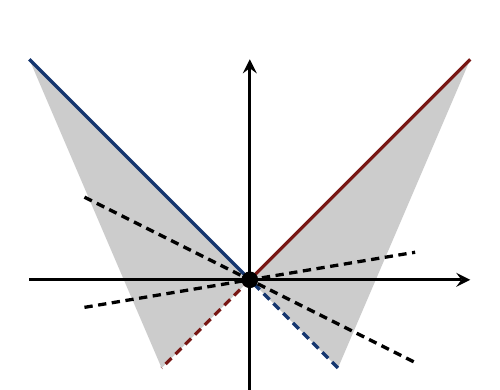
\begin{tikzpicture}[scale=1.4]
            % basics
            \draw [-stealth,color=black,very thick] (2,-1) -- (2,2);
            \draw [-stealth,color=black,very thick] (0,0) -- (4,0);
            \draw [name path = neg_up, color = myblue, very thick] (0,2) -- (2,0);
            \draw [name path = pos_up, color = myred, very thick] (2,0) -- (4,2);
            \draw [name path = pos_down, color = myblue, very thick, densely dashed] (2.8,-0.8) -- (2,0);
            \draw [name path = neg_down, color = myred, very thick, densely dashed] (2,0) -- (1.2,-0.8);
            \filldraw [color=black] (2,0) circle (2pt);
            \draw [color = black, very thick, densely dashed] (0.5,-0.25) -- (3.5,0.25);
            \draw [color = black, very thick, densely dashed] (0.5,0.75) -- (3.5,-0.75);
            \tikzfillbetween[of=neg_up and neg_down, on layer=bg]{black!20!white};
            \tikzfillbetween[of=pos_up and pos_down, on layer=bg]{black!20!white};
        \end{tikzpicture}

        L1-norm (1-dimension)
\end{minipage}
\hfill
\begin{minipage}{0.45\textwidth}
    For each component of the vector of the L-1 norm $f(\beta_j) = \lvert \beta_j \rvert$, we have:
    \begin{itemize}
        \item[-] \textcolor{myred}{$\beta_j>0$: $f'(\beta_j) = 1$}
        \item[-] \textcolor{myblue}{$\beta_j<0$: $f'(\beta_j) = -1$}
        \item[-] $\beta_j=0$: $\mathrm{d}f \in [-1,1]$ (shaded area)
    \end{itemize}
    which gives the results stated above.
\end{minipage}

Take another look at this result 
\begin{proposition}{Lasso Parameter Selection Rule}{lasso-math}
    $$
    \frac{1}{n} \mathbf{X}'  \left(\mathbf{y}-\mathbf{X}\boldsymbol{\beta} \right) =\frac{1}{n} \mathbf{X}'\boldsymbol{\epsilon}  = \lambda \begin{cases}
        \mathrm{sign}\left(\beta_j\right), & \beta_j\neq 0\\
        \left[ -1,1 \right], & \beta_j =0
    \end{cases}
    $$
    which gives a parameter selection criterion: for $\beta_j \neq 0$, \myhl[myred]{$\mathrm{sign}(\beta_j)$ \textbf{must agree} with $\mathrm{Corr}(\mathbf{x}_j,\boldsymbol{\epsilon})$}, the correlation between the $j$-th variable $\mathbf{x}_j$ and (full-model) residuals $\boldsymbol{\epsilon}=\mathbf{y}-\mathbf{X}\boldsymbol{\beta}$.
\end{proposition}

\subsection{Algorithm: LARS}
Mathematically, Lasso is quite intuitive, but computationally, it can be quite consuming. \citet{efron2004least} propose an algorithm that takes steps from a all-0 model to the biggest model (OLS), that is, \textbf{Least Angle Regression (LARS)}. 

\subsubsection*{Intuition}
The basic intuition of LARS is quite straight-forward: covariates are considered from the \myhl[myred]{\textbf{\textit{highest}}} corerlation with $\mathbf{y}$ (\textit{smallest} angle from $\mathbf{y}$) to the \myhl[myblue]{\textbf{\textit{least}}} correlated one (\textit{largest} angle from $\mathbf{y}$) (illustrated below).

\begin{figure}[ht]
    \begin{minipage}[b]{0.45\textwidth}
    \centering
      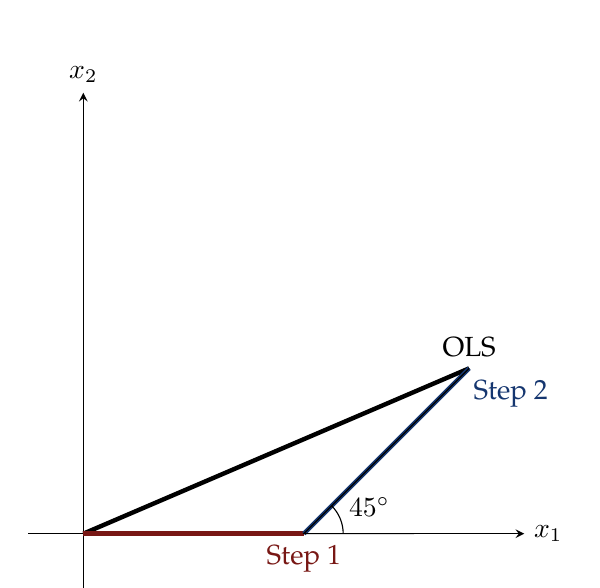
\begin{tikzpicture}[scale=1.4]
          % basics
          \draw [-stealth,color=black,thin] (-0.5,0) -- (4,0) node[right] {$x_1$};
          \draw [-stealth,color=black,thin] (0,-0.5) -- (0,4) node[above] {$x_2$};
          \draw [color=black, ultra thick] (0,0) -- (3.5,1.5) node[above] {OLS};
          \draw [color=myred, ultra thick] (0,0) -- (2,0) node[below] {Step 1};
          \draw [color=myblue, ultra thick] (2,0) -- (3.5,1.5) node[below,xshift=15pt] {Step 2};
          
          \coordinate (X) at (3.5,1.5);
            \coordinate (A) at (2,0);
            \coordinate (Y) at (3,0);

            % Draw Angle
            \draw[thin] (Y) -- (A) -- (X)
            pic ["$45^{\circ}$", draw, thin, angle eccentricity=1.8] {angle = Y--A--X};
      \end{tikzpicture}
    \end{minipage}
    \hfill
    \begin{minipage}[b]{0.45\textwidth}
        \centering
        \tdplotsetmaincoords{60}{45}
        \begin{tikzpicture}
            [scale=5,
                tdplot_main_coords,
                axis/.style={-stealth,black,thin},
                vector/.style={black,very thick},
                LARS/.style={ultra thick}]

            %standard tikz coordinate definition using x, y, z coords
            \coordinate (O) at (0,0,0);
            
            \coordinate (P) at (0.8, 0.6, 0.2);

            \coordinate (P12) at (0.8, 0.6, 0);
            \coordinate (P23) at (0, 0.6, 0.2);
            \coordinate (P13) at (0.8, 0, 0.2);
            \coordinate (P1) at (0.8, 0, 0);
            \coordinate (P2) at (0, 0.6, 0);
            \coordinate (P3) at (0, 0, 0.2);
            
            %draw axes
            \draw[axis] (0,0,0) -- (1,0,0) node[anchor=north east]{$x_1$};
            \draw[axis] (0,0,0) -- (0,1,0) node[anchor=north west]{$x_2$};
            \draw[axis] (0,0,0) -- (0,0,1) node[anchor=south]{$x_3$};

            % projection dash line
            \draw[thin, black, densely dashed] (P12)--(P1);
            \draw[thin, black, densely dashed] (P12)--(P2);
            \draw[thin, black, densely dashed] (P)--(P13);
            \draw[thin, black, densely dashed] (P)--(P23);
            \draw[thin, black, densely dashed] (P23)--(P3);
            \draw[thin, black, densely dashed] (P13)--(P3);
            \draw[thin, black, densely dashed] (P23)--(P2);
            \draw[thin, black, densely dashed] (P13)--(P1);
            \draw[thin, black, densely dashed] (P)--(P12);
            
            %draw a vector from O to P
            \draw[vector] (O) -- (P);

            % draw LARS steps
            \draw[LARS, myred] (O) -- (0.2,0,0) node[left,xshift=-10pt] {Step 1};
            \draw[LARS, myblue] (0.2,0,0) -- (0.6,0.4,0) node[below] {Step 2};
            \draw[LARS, teal] (0.6,0.4,0) -- (P) node[right] {Step 3};

            % approaching, but not exactly reach OLS
            %\draw[thin, teal, densely dashed] (P13)--(0.8,0.35,0.2);
            %\draw[thin, teal, densely dashed] (0.8,0.35,0.2)--(0,0.35,0.2);
        \end{tikzpicture}
    \end{minipage}
\end{figure}

And the steps of the LARS algorithm are
\begin{itemize}
    \item[1] start with the null model $\hat{\boldsymbol{\beta}}=\mathbf{0}$: $\hat{\boldsymbol{\mu}} = \mathbf{X}'\mathbf{0}=\mathbf{0}$ 
    \item[2] calculate residual vector $\mathbf{r} = \mathbf{y}-\hat{\boldsymbol{\mu}}$
    \item[3] determine the correlation vector between $\mathbf{r}$ and each parameter $\mathbf{x}_j,\forall j=1,\cdots,p$: $\mathbf{X}'\mathbf{r}$
    \item[4] pick the largest correlation $\mathbf{x}^*_{\text{step}1,1}$, increase its $\hat{{\beta}}$ to the point where its correlation with $\mathbf{r}$ will be \myhl[red!55!black]{\textbf{equal}} with that of another parameter $\mathbf{x}^*_{\text{step1},2}$ 
    \item[5] next, increase the $\hat{\beta}$ for both $\mathbf{x}^*_{\text{step1},1},\mathbf{x}^*_{\text{step1},2}$ in an \myhl[red!55!black]{\textbf{equiangular}} direction between these two, until a third parameter becomes equally important
\end{itemize}
And keep looping this way, until all the predictors enter the model and eventually $\mathbf{X}'\mathbf{r}=\mathbf{0}$

\subsubsection*{Properties of LARS}
LARS has several properties:
\begin{itemize}
    \item geometrically travels in the direction of \textbf{equal} angle to all active covariates
    \item assume all covariates are independent
    \item computationally quick: only take $m$ steps, where $m$ is the number of parameters being considered
\end{itemize}
And it is in between 2 classic model-selection methods: \textbf{Forward Selection} and \textbf{Stagewise Selection}:
\begin{itemize}
    \item \myhl[red!55!black]{\textbf{Forward Selection}}
    \begin{itemize}
        \item for $\mathbf{y}$, select the most correlated $\mathbf{x}_{j_1}$
        \item regress $\mathbf{x}_{j_1}$ on $\mathbf{y}$, get the residuals
        \item select the most correlated $\mathbf{x}_{j_2}$ with the redisual of $\mathbf{y}$ net of $\mathbf{x}_{j_1}$
    \end{itemize}
    looping this, for a $k-$parameter linear model, it takes $k$ steps. Forward Selection is an aggressive fitting technique, can be overly greedy (some important predictors may be eliminated due to correlation with already selected variables).
    \item \myhl[red!55!black]{\textbf{Forward Stagewise}}
    \begin{itemize}
        \item also begin with $\hat{\boldsymbol{\mu}}=0$
        \item for a current Stagewise estimate $\hat{\boldsymbol{\mu}}$, the current residual vector is then $\mathbf{y}-\hat{\boldsymbol{\mu}}$, its correlation with $\mathbf{X}$ is then  $\mathbf{X'}(\mathbf{y}-\hat{\boldsymbol{\mu}})\equiv \hat{\mathbf{c}}$
        \item next, heavily computational, go in the direction of the greatest current correlation, but by only a \myhl[red!55!black]{\textbf{small}} step $$ \hat{j}= \arg\max\lvert \hat{c}_j \rvert, \ \hat{\boldsymbol{\mu}}\rightarrow \hat{\boldsymbol{\mu}}+\epsilon\cdot \mathrm{sign}(\hat{c}_{\hat{j}})\cdot \mathbf{x}_{\hat{j}} $$
        here, $\epsilon$ is a \textbf{small} constant, hence avoiding the greediness of Forward Selection, at a cost of computational efficiency\footnote{Forward Selection is essentially choosing $\epsilon=\lvert \hat{c}_{\hat{j}} \rvert$}.
    \end{itemize}
\end{itemize}
LARS avoids the over-greediness of Forward Selection and computational heaviness of Forward Stagewise.

\subsection{From LARS to Lasso}
The Lasso algorithm is built upon LARS, with the constraint from the mathematical condition of Proposition \ref{prop:lasso-math}: \myhl[myblue]{$\mathrm{sign}(\beta_j)$ \textbf{must agree} with $\mathrm{Corr}(\mathbf{x}_j,\boldsymbol{\epsilon})$}. 

\begin{theorem}{Lasso Modification Condition}{lasso-modif}
    If $\tilde{\gamma}< \hat{\gamma}$, stop the onging LARS step at $\gamma = \tilde{\gamma}$ and remove $j$ from the calculation of the next equiangular direction, where
    \begin{itemize}
        \item the path at any LARS step is $$\boldsymbol{\beta}(\gamma),\ \beta_j(\gamma) = \hat{\beta}_j + \gamma\hat{d}_j$$ $\hat{d}_j$ specifies the \myhl[blue!45!black]{\textbf{direction}} to take the $j$-th component, $\gamma$ is \myhl[blue!45!black]{\textbf{how far}} to travel in the direction of $\hat{d}_j$ before adding in a new covariate
        \item $\hat{\gamma}$ represents the smallest \myhl[red!55!black]{\textbf{positive}} value of $\gamma$ s.t. some new covariate joins the active set (the set of covariates used on path)
        \item $\tilde{\gamma}$ represents the first time $\beta_j(\gamma)$ \myhl[red!55!black]{\textbf{changes signs}}.
    \end{itemize}
\end{theorem}
The key point of \ref{thm:lasso-modif} is that Lasso does \textbf{NOT} allow the $\hat{\beta}_j$ to change signs, if it changes sign, it will be substracted from the active set. Now, from this point of view, we can compare the 3 algorithms:

\begin{center}
    \begin{tabular}{ r|l } 
     \hline
     LARS & no sign restrictions  \\ 
     Lasso &  $\hat{\beta}_j$ agrees in sign with $\hat{c}_j$ \\
     Stagewise & successive differences of $\hat{\beta}_j $ agree in sign with the current correlation $\hat{c}=\mathbf{x}_j'(\mathbf{y}-\hat{\boldsymbol{\mu}})$\\
     \hline
    \end{tabular}
\end{center}

Again, LARS requires the least steps but is most greedy, Stagewise is computationally consuming but robust. Lasso is in between.

\section{Consistency of Lasso}
Next, we want to establish the consistency of Lasso, by showing that Lasso selects exactly the relevant covariates asymptotically. We do this in 2 steps:
\begin{itemize}
    \item show that Lasso at least captures all the relevant covariates
    \item asymptotically, under some conditions, Lasso selects exactly all the relevant covariates, not more
\end{itemize}

\subsection{Overestimation}
First, Lasso tends to select a superset of the relevant covariates.

Define the true relevant set Lasso selection estimation $\hat{S}_0$ aim to select as
    $$ S_0 = \left\{ j:\beta^0_j \neq 0,j \neq 1,\cdots,p \right\} $$
    and for some $C>0$, define the relevant set w.r.t. $C$ as $$ S_0^{\text{relevant}(C)} = \left\{ j: \lvert \beta^0_j \rvert \geq C, j=1,\cdots,p \right\} $$ then we have
\begin{theorem}{Lasso Overestimation Condition}{lasso-overest}
    $\forall 0<C<\infty$ $$ \mathbb{P}\left[ \hat{S}_0(\lambda) \supset S_0^{\text{relevant}(C)} \right] \xrightarrow{n\rightarrow \infty}1 $$
\end{theorem}

\subsection*{Consistency}
The consistency of Lasso is established by \citet{meinshausen2006variable} as
\begin{theorem}{Consistency of Lasso}{lasso_consistency}
    For a suitable $\lambda = \lambda_n \gg \sqrt{s_0\log(p)/n}$, Lasso is consistent, i.e. $$ \mathbb{P}\left[ \hat{S}(\lambda)=S_0 \right] \xrightarrow{n\rightarrow\infty}1 $$
    if and only if it satisfies the 2 properties:
    \begin{itemize}
        \item $\beta-$min condition (unselected coefficients non-trivial): $\inf_{j\in S^c_0}\lvert \beta^0_j \rvert \gg \sqrt{s_0 \log(p)/n}$
        \item \myhl[blue!45!black]{\textbf{irrepresentable} condition}: $\mathbf{X}$ should \textbf{NOT} exhibit too strong a degree of linear dependence w.r.t. the selected covariates, that is, for some $0<\theta<1$ $$ \left\Vert \hat{\Sigma}_{2,1}\hat{\Sigma}_{1,1}^{-1}\mathrm{sign}\left( \beta^0_1,\cdots,\beta^0_{s_0}\right) \right\Vert _{\infty} \leq\theta $$
    \end{itemize}
\end{theorem}

\paragraph*{discussion on the irrepresentable condition} denote $\hat{\Sigma}=n^{-1}\mathbf{XX}'$, and let the active set $S_0=\left\{ j:\beta^0_j\neq 0 \right\}=\left\{ 1,\cdots, s_0 \right\}$ consists of the first $s_0$ variables, let 
$$ \hat{\Sigma} = \left( \begin{matrix}
    \hat{\Sigma}_{1,1} & \hat{\Sigma}_{1,2} \\
    \hat{\Sigma}_{2,1} & \hat{\Sigma}_{2,2}
\end{matrix} \right) $$
where $\hat{\Sigma}_{1,1}$ is a $s_0\times s_0$ var-cov matrix of the active variables $\mathbf{X}_1$, $\hat{\Sigma}_{2,2}$ is a $(p-s_0)\times (p-s_0)$ cov-var matrix of the other variables $\mathbf{X}_2$\footnote{Here, $\mathbf{X}_1$ is $n\times s_0$, $\mathbf{X}_2$ is $n\times p-s_0$}, then for a Lasso estimation $\hat{\boldsymbol{\beta}}$ that assign non-zero coefficients \textbf{only} to $\mathbf{X}_1$, we can, following the Lasso result in Proposition \ref{prop:lasso-math}, have\sidenotes{$ \lVert \cdot \rVert$ is the \\ component-wise \\ max-norm}
\begin{equation}\label{eq:lasso_consist}
    \begin{aligned}
        \frac{1}{n}\mathbf{X}'\left(\mathbf{y}-\mathbf{X}\hat{\boldsymbol{\beta}}\right) &= \lambda \cdot \mathrm{sign}(\hat{\boldsymbol{\beta}}_1) & \Rightarrow \frac{1}{n}\mathbf{X}_1'\left(\mathbf{y}-\mathbf{X}_1\hat{\boldsymbol{\beta}}_1\right) &= \lambda \cdot \mathrm{sign}(\hat{\boldsymbol{\beta}}_1) \\
        \lVert \frac{1}{n}\mathbf{X}_2'\left(\mathbf{y}-\mathbf{X}\hat{\boldsymbol{\beta}}\right) \rVert _{\infty} &\leq \lambda & \Rightarrow \lVert \frac{1}{n}\mathbf{X}_2'\left(\mathbf{y}-\mathbf{X}_1\hat{\boldsymbol{\beta}}_1\right) \rVert _{\infty} &\leq \lambda
    \end{aligned}
\end{equation}
Now, let's assume $ \mathrm{supp}(\hat{\boldsymbol{\beta}}) = \mathrm{supp}(\boldsymbol{\beta}) = S_0 $, then the true model is
$$
\mathbf{y} = \mathbf{X}\boldsymbol{\beta} + \boldsymbol{\epsilon} = \begin{bmatrix}
    \mathbf{X}_1 &\mathbf{X}_2
\end{bmatrix}\cdot \begin{bmatrix}
    \boldsymbol{\beta}_1 \\ \mathbf{0}
\end{bmatrix} + \boldsymbol{\epsilon} = \mathbf{X}_1\boldsymbol{\beta}_1+\boldsymbol{\epsilon}
$$
Put this back to the results in Equation \ref{eq:lasso_consist}, we have
\begin{itemize}
    \item for the selected covariates $\mathbf{X}_1$ 
    \begin{align*}
        &\frac{1}{n}\mathbf{X}_1'\left(\mathbf{y}-\mathbf{X}_1\hat{\boldsymbol{\beta}}_1\right) = \lambda \cdot \mathrm{sign}(\hat{\boldsymbol{\beta}}_1)\\
        \Rightarrow & \frac{1}{n}\mathbf{X}_1'\left(\mathbf{X}_1\boldsymbol{\beta}_1+\boldsymbol{\epsilon}-\mathbf{X}_1\hat{\boldsymbol{\beta}}_1\right) = \lambda \cdot \mathrm{sign}(\hat{\boldsymbol{\beta}}_1)\\
        \Rightarrow & \frac{1}{n}\mathbf{X}_1' \mathbf{X}_1 \left( \hat{\boldsymbol{\beta}}_1- \boldsymbol{\beta}_1\right) = \frac{1}{n}\mathbf{X}_1'\boldsymbol{\epsilon}- \lambda \cdot \mathrm{sign}(\hat{\boldsymbol{\beta}}_1) \\
        \Rightarrow & \hat{\boldsymbol{\beta}}_1- \boldsymbol{\beta}_1 = \left( \frac{1}{n}\mathbf{X}_1' \mathbf{X}_1 \right)^{-1} \left[ \frac{1}{n}\mathbf{X}_1'\boldsymbol{\epsilon}- \lambda \cdot \mathrm{sign}(\hat{\boldsymbol{\beta}}_1) \right] \\
        \Rightarrow & \hat{\boldsymbol{\beta}}_1 = \boldsymbol{\beta}_1 + \left( \frac{1}{n}\mathbf{X}_1' \mathbf{X}_1 \right)^{-1} \frac{1}{n}\mathbf{X}_1'\boldsymbol{\epsilon} -  \underbrace{\left( \frac{1}{n}\mathbf{X}_1' \mathbf{X}_1 \right)^{-1} \lambda \cdot \mathrm{sign}(\hat{\boldsymbol{\beta}}_1)}_{\text{L1-norm regularization}}
    \end{align*}
    \item for the non-selected covariates $\mathbf{X}_2$\footnote{Here, additionally assume \myhl[myred]{\textbf{sign consistency}}: \begin{align*} \mathrm{sign}(\hat{\beta}_j)&=\mathrm{\beta_j}\neq 0, \forall j\in S_0 &\text{selected coviates} \\ \mathrm{sign}(\hat{\beta}_j)&=\mathrm{\beta_j}= 0, \forall j\in S_0^C &\text{non-selected coviates} \end{align*} }
    \begin{align*}
        & \left\Vert \frac{1}{n}\mathbf{X}_2'\left(\mathbf{y}-\mathbf{X}_1\hat{\boldsymbol{\beta}}_1\right) \right\Vert _{\infty} \leq \lambda \\
        \Rightarrow & \left\Vert \frac{1}{n}\mathbf{X}_2'\left[ \mathbf{X}_1 \left(\hat{\boldsymbol{\beta}}_1- \boldsymbol{\beta}_1\right) -\boldsymbol{\epsilon} \right] \right\Vert _{\infty} \leq \lambda \\
        \Rightarrow & \left\Vert \frac{1}{n}\mathbf{X}_2'\left\{ \mathbf{X}_1 \left[ \left( \frac{1}{n}\mathbf{X}_1' \mathbf{X}_1 \right)^{-1} \frac{1}{n}\mathbf{X}_1'\boldsymbol{\epsilon} - \left( \frac{1}{n}\mathbf{X}_1' \mathbf{X}_1 \right)^{-1} \lambda \cdot \mathrm{sign}(\hat{\boldsymbol{\beta}}_1) \right] -\boldsymbol{\epsilon} \right\} \right\Vert _{\infty} \leq \lambda \\
        \xRightarrow{\text{assume sign consistency}} & \left\Vert \frac{1}{n}\mathbf{X}_2' \mathbf{X}_1 \left[ \left( \frac{1}{n}\mathbf{X}_1' \mathbf{X}_1 \right)^{-1} \frac{1}{n}\mathbf{X}_1'\boldsymbol{\epsilon} - \left( \frac{1}{n}\mathbf{X}_1' \mathbf{X}_1 \right)^{-1} \lambda \cdot \textcolor{myred}{\mathrm{sign}({\boldsymbol{\beta}}_1)} \right]  - \frac{1}{n}\mathbf{X}_2'\boldsymbol{\epsilon} \right\Vert _{\infty} \leq \lambda 
    \end{align*}
    if we assume $\boldsymbol{\epsilon}\sim \mathcal{N}(\mathbf{0},\sigma^2 \mathbf{I}_n)$, i.e., $\epsilon_i$ i.i.d. $\sim \mathcal{N}({0},\sigma^2)$, and for each variable in the design matrix, we also assume standard normal $\mathbf{x}_j\sim \mathcal{N}(\mathbf{0},\mathbf{I}_n)$ (think this as normalizing each variable), then we have 
    $$
    \frac{1}{n}\mathbf{x}_j'\boldsymbol{\epsilon}\sim \mathcal{N}\left(0,\frac{\sigma^2}{n}\right),\forall j=1,\cdots,p
    $$
    and also $ \max_{1\leq j\leq p}\mathbf{x}_j \sim \sqrt{2\log p}$. This gives
    $$
    \left\Vert \frac{1}{n}\mathbf{X}'\boldsymbol{\epsilon} \right\Vert _{\infty} \sim \sqrt{2 \log p}\cdot \frac{\sigma}{\sqrt{n}} = \sqrt{\frac{2\log p}{n}}\sigma
    $$
    hence, it can be bounded by $\lambda = \sqrt{\frac{C\log p}{n}}\sigma $, where the constant $C\geq 2$, then with large probability
    $$
    \left\Vert \frac{1}{n}\mathbf{X}'\boldsymbol{\epsilon} \right\Vert _{\infty} \leq \frac{1}{3}\lambda \Rightarrow \begin{aligned}
        \left\Vert \frac{1}{n}\mathbf{X}'_1\boldsymbol{\epsilon} \right\Vert _{\infty} &\leq \frac{1}{3}\lambda \\
        \left\Vert \frac{1}{n}\mathbf{X}'_2\boldsymbol{\epsilon} \right\Vert _{\infty} &\leq \frac{1}{3}\lambda 
    \end{aligned}
    $$
    now go back to the condition of non-selected covariates $\mathbf{X}_2$
    \begin{align*}
         & \left\Vert \frac{1}{n}\mathbf{X}_2' \mathbf{X}_1 \left[ \left( \frac{1}{n}\mathbf{X}_1' \mathbf{X}_1 \right)^{-1} \frac{1}{n}\mathbf{X}_1'\boldsymbol{\epsilon} - \left( \frac{1}{n}\mathbf{X}_1' \mathbf{X}_1 \right)^{-1} \lambda \cdot \textcolor{myred}{\mathrm{sign}({\boldsymbol{\beta}}_1)} \right]  - \frac{1}{n}\mathbf{X}_2'\boldsymbol{\epsilon} \right\Vert _{\infty} \\
        \leq & \left\Vert \frac{1}{n}\mathbf{X}_2' \mathbf{X}_1 \left( \frac{1}{n}\mathbf{X}_1' \mathbf{X}_1 \right)^{-1} \frac{1}{n}\mathbf{X}_1'\boldsymbol{\epsilon} \right\Vert _{\infty}  +  \left\Vert \frac{1}{n}\mathbf{X}_2' \mathbf{X}_1  \left( \frac{1}{n}\mathbf{X}_1' \mathbf{X}_1 \right)^{-1}{\mathrm{sign}({\boldsymbol{\beta}}_1)} \right\Vert _{\infty}\cdot \lambda + \left\Vert \frac{1}{n}\mathbf{X}_2'\boldsymbol{\epsilon} \right\Vert _{\infty} \\
        \leq & \left\Vert \frac{1}{n}\mathbf{X}_2' \mathbf{X}_1 \left( \frac{1}{n}\mathbf{X}_1' \mathbf{X}_1 \right)^{-1} \right\Vert _{\infty} \cdot \underbrace{\left\Vert \frac{1}{n}\mathbf{X}_1'\boldsymbol{\epsilon} \right\Vert _{\infty}}_{\leq \frac{1}{3}\lambda}  +  \left\Vert \frac{1}{n}\mathbf{X}_2' \mathbf{X}_1  \left( \frac{1}{n}\mathbf{X}_1' \mathbf{X}_1 \right)^{-1} \right\Vert _{\infty} \cdot \underbrace{\left\Vert {\mathrm{sign}({\boldsymbol{\beta}}_1)}\right\Vert _{\infty}}_{= 1} \cdot \lambda +  \underbrace{\left\Vert \frac{1}{n}\mathbf{X}_2'\boldsymbol{\epsilon} \right\Vert _{\infty}}_{\leq \frac{1}{3}\lambda}\\
        \leq & \left\Vert \frac{1}{n}\mathbf{X}_2' \mathbf{X}_1 \left( \frac{1}{n}\mathbf{X}_1' \mathbf{X}_1 \right)^{-1} \right\Vert _{\infty} \cdot \frac{4}{3}\lambda + \frac{1}{3}\lambda \textcolor{myred}{\leq \lambda}
    \end{align*}
    for the last part ($\leq \lambda$) to stand, a necessary condition is $\left\Vert \mathbf{X}_2' \mathbf{X}_1 \left( \mathbf{X}_1' \mathbf{X}_1 \right)^{-1} \right\Vert _{\infty} \leq \frac{1}{2}$, or more generally, the \myhl[myred]{\textbf{irrepresentable condition}}:
    \begin{align*}
        \left\Vert \mathbf{X}_2' \mathbf{X}_1 \left( \mathbf{X}_1' \mathbf{X}_1 \right)^{-1} \cdot \mathrm{sign}(\boldsymbol{\beta}_1) \right\Vert \leq \left\Vert \mathbf{X}_2' \mathbf{X}_1 \left( \mathbf{X}_1' \mathbf{X}_1 \right)^{-1} \right\Vert _{\infty}\cdot \left\Vert \mathrm{sign}(\boldsymbol{\beta}_1) \right\Vert = \left\Vert \hat{\Sigma}_{2,1}\hat{\Sigma}_{1,1}^{-1}\mathrm{sign}\left( \beta^0_1,\cdots,\beta^0_{s_0}\right) \right\Vert _{\infty} \leq\theta
    \end{align*}
\end{itemize}
The idea of \myhl[myred]{\textit{\textbf{irrepresentable}}} is that the \textbf{maximum} correlation between \underline{noise features} and important variables needs to be \myhl[myred]{\textbf{bounded}}.

\subsection{Oracle}
Consistency is part of the requirements of an oracle procedure
\begin{definition}{Oracle Property}{oracle}
    For a fitting procedure $\delta$, and the estimation $\hat{\beta}(\delta)$, then if $\delta$ is an oracle procedure if $\hat{\beta}(\delta)$ asymptotically has the following properties 
    \begin{itemize}
        \item \myhl[red!55!black]{\textbf{consistency}} (identifying right subset model): $\left\{ j:\hat{\beta}_j \neq 0 \right\} = S_0$
        \item \myhl[red!55!black]{\textbf{optimal estimation rate}} (asymptotically normal): $\sqrt{n}\left( \beta(\delta)_{S_0} - \beta^0_{S_0} \right) \xrightarrow{d} \mathcal{N}(0,\Sigma_0)$, where $\Sigma_0$ is the \textit{true} subset covariance matrix
    \end{itemize}
\end{definition}
The oracle property gives consistency, and asymptotic normality. Ideally, this is what you need.


\section{Variants of Lasso}
Lasso is great, but there is still space for improvement
\begin{itemize}
    \item for high dimension $p>n$ cases, lasso selects \myhl[myred]{\textbf{at most}} $n$ variables 
    \item for a group of variables with large \myhl[myred]{\textbf{pairwise correlation}}, then the lasso tends to select \textbf{only one}
    \item for $n>p$ cases, if there are high correlations between predictors, lasso is dominated by ridge regression
\end{itemize}
Here are some popular variants people came up with to tackle these issues.

\subsection{Adaptive Lasso}
Adaptive Lasso replaces the $L_1-$penalty for a \myhl[myblue]{\textbf{re-weighted}} version:
\begin{align*}
    \hat{\boldsymbol{\beta}}(\lambda) = \arg\min_{\boldsymbol{\beta}} \left( \frac{1}{n} \left\Vert \mathbf{y}-\mathbf{X}\boldsymbol{\beta} \right\Vert ^2_2 + \lambda_n \sum^p_{j=1}\frac{\lvert \beta_j \rvert}{ \lvert \hat{\beta}_{init,j} \rvert^{\gamma} } \right)
\end{align*}
this is a 2-step procedure:
\begin{itemize}
    \item Step 1: run an initial estimation (could be OLS or Lasso) as $\hat{\boldsymbol{\beta}}_{init}$, if $\hat{\beta}_{init,j}=0$, then $\hat{\beta}_{adapt,j}=0$
    \item Step 2: run the reweighted estimation, which is still an $L1-$penalization, still a \textbf{convex} optimization problem (allowing the same Lasso algorithm to solve)
\end{itemize}
\begin{theorem}{Properties of Adaptive Lasso}{adapt_lasso}
    The adaptive Lasso has the following properties
    \begin{itemize}
        \item If $\lvert \hat{\beta}_{init,j} \rvert$ is large (\textit{important} features), then the adaptive Lasso uses a small penalty
        \item The adaptive lasso enjoys the oracle properties 
        \begin{itemize}
            \item \myhl[myblue]{\textbf{consistency}}: $\lim_n \mathbb{P}\left(\hat{S}(\lambda)=S_0\right)=1$
            \item \myhl[myblue]{\textbf{asymptotic normality}}: $\sqrt{n}\left(\beta_{S_0}-\beta^*_{S_0}\right) \xrightarrow{d} \mathcal{N}(0,\sigma^2\times C^{-1}_{1,1}) $
        \end{itemize}
        if $\lambda_n$ is chosen properly, i.e., $\frac{\lambda_n}{\sqrt{n}}\rightarrow 0$ and $\lambda_n n^{(\gamma-1)/2}\rightarrow \infty$. Notice: the adaptive lasso's consistency \myhl[myred]{\textbf{DOES NOT}} require the irrepresentable condition.
    \end{itemize}

\end{theorem}

\subsection{Naive Elastic Net}
The idea is to do a convex combination of Lasso and Ridge: $\forall \lambda_1,\lambda_2 \geq 0$, the naive elastic net criterion is
\begin{align*}
    \mathcal{L}(\lambda_1,\lambda_2,\boldsymbol{\beta}) = \lVert \mathbf{y}-\mathbf{X}\boldsymbol{\beta} \rVert _2^2 + \lambda_1 \underbrace{\lVert \boldsymbol{\beta} \rVert _1}_{=\sum^p_{j=1}\lvert \beta_j \rvert} + \lambda_2 \underbrace{\lVert \boldsymbol{\beta} \rVert^2_2}_{=\sum^p_{j=1} \beta_j^2}
\end{align*}
Now, notice that both $\lVert \mathbf{y}-\mathbf{X}\boldsymbol{\beta} \rVert _2^2$ and $\lVert \boldsymbol{\beta} \rVert^2_2$ are both \textbf{quadratic}, hence, we can reframe the qeustion as a lasso-type optimization, with an augmented data $(\mathbf{X}^*,\mathbf{y}^*)$ where 
\begin{align*}
    \mathbf{X}^*_{(n+p)\times p} &= \frac{1}{\sqrt{1+\lambda_2}} \begin{pmatrix} \mathbf{X} \\ \sqrt{\lambda_2}\mathbf{I} \end{pmatrix} & \mathbf{y}^*_{n+p} =  \begin{pmatrix} \mathbf{y} \\ \mathbf{0} \end{pmatrix}
\end{align*}
then we have 
\begin{definition}{Naive elastic net solution}{naive_elastic_net}
    Let $\gamma = \frac{\lambda_1}{\sqrt{1+\lambda_2}}$, then the naive elastic net criterion can be rewritten as
    $$
    \mathcal{L}(\gamma,\boldsymbol{\beta}) = \mathcal{L}(\gamma,\boldsymbol{\beta}^*) = \lVert \mathbf{y}^*-\mathbf{X}^*\boldsymbol{\beta}^* \rVert _2^2 + \gamma \lVert \boldsymbol{\beta}^* \rVert _1 
    $$
    which gives use the estimation for the augmented data
    $$
    \hat{\boldsymbol{\beta}}^* = \arg\min_{\boldsymbol{\beta}^*} \mathcal{L}(\gamma,\boldsymbol{\beta}^*)
    $$
    and the estimation for the true model of the original data $(\mathbf{X},\mathbf{y})$ is 
    $$
    \hat{\boldsymbol{\beta}} = \frac{1}{\sqrt{1+\lambda_2}}\hat{\boldsymbol{\beta}}^*
    $$
\end{definition}
Naive elastic net enjoys 2 advantages:
\begin{itemize}
    \item The estimation is done on the augemented data $(\mathbf{X}^*,\mathbf{y}^*)$, and now $\mathbf{X}^*$ is $(n+p)\times p$, therefore, $\mathrm{rank}(\mathbf{X}^*)=p$, hence all $p$ predictors \textbf{can} be selected, instead of just $n$, like in Lasso.
    \item Computationally, it is similarly efficient as Lasso
\end{itemize}

If we further assume an orthogonal design ($\mathbf{X}'\mathbf{X}=\mathbf{I}_p$), we can easily compare the 3 estimations
\begin{align*}
    \hat{{\beta}}_j\left(\text{naive elastic net}\right) &= \frac{\left( \left\vert \hat{\beta}_j^{OLS}\right\vert -\frac{\lambda_1}{2} \right)_+}{1+\lambda_2} \cdot \mathrm{sign}\left[ \hat{\beta}_j^{OLS}\right] \\
    \hat{{\beta}}_j\left(\text{ridge}\right) &= \frac{\hat{\beta}_j^{OLS}}{1+\lambda_2}\\
    \hat{\beta}_j \left(\text{lasso}\right) &= \left( \left\vert \hat{\beta}_j^{OLS}\right\vert -\frac{\lambda_1}{2} \right)_+\cdot \mathrm{sign}\left[ \hat{\beta}_j^{OLS}\right]
\end{align*}

This comparison is illustrated graphically below.

\begin{figure}[ht]
    \centering
    \begin{minipage}[b]{0.45\textwidth}
    \centering
      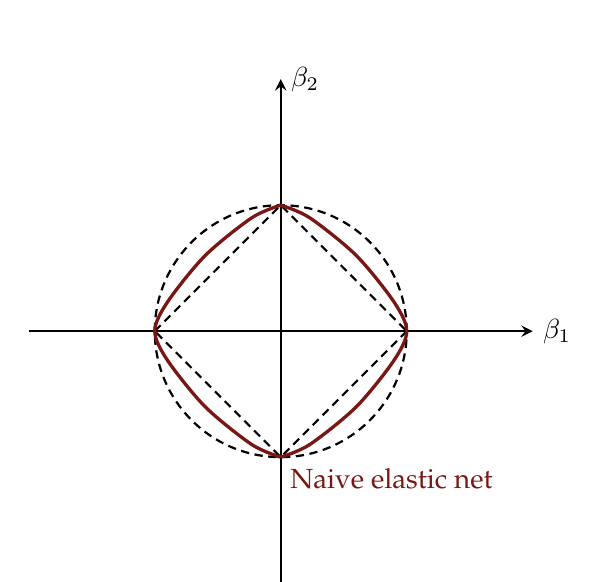
\begin{tikzpicture}[scale=1.6]
          % basics
          \draw [-stealth,color=black,thick] (0,2) -- (4,2) node[right]{$\beta_1$};
          \draw [-stealth,color=black,thick] (2,0) -- (2,4) node[right]{$\beta_2$};
          \draw [color=black,thick, densely dashed] (1,2) -- (2,3) -- (3,2);
          \draw [color=black,thick, densely dashed]  (3,2) -- (2,1) -- (1,2);
          \draw [color=black, thick, densely dashed] (1,2) -- (3,2);
          \node[circle,draw,minimum size=3.2cm, thick, densely dashed] (c) at (2,2){};
          \draw [color=myred, very thick] plot [smooth] coordinates {(2,3) (2.23,2.9) (2.6,2.6) (2.9,2.23) (3,2) (2.9,1.77) (2.6,1.4) (2.23,1.1) (2,1)} node[below,xshift=40pt]{Naive elastic net};
          \draw [color=myred, very thick] plot [smooth] coordinates {(2,3) (1.77,2.9) (1.4,2.6) (1.1,2.23) (1,2) (1.1,1.77) (1.4,1.4) (1.77,1.1) (2,1)};
      \end{tikzpicture}
    \end{minipage}
    \hfill
    \begin{minipage}[b]{0.45\textwidth}
        \centering
        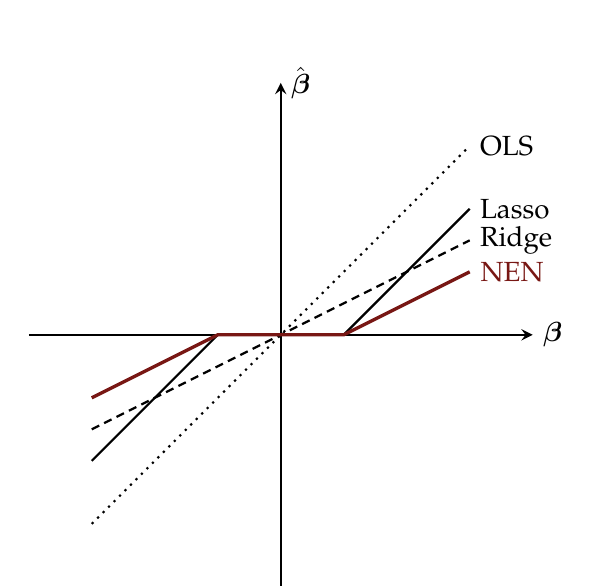
\begin{tikzpicture}[scale=1.6]
            % basics
            \draw [-stealth,color=black,thick] (0,2) -- (4,2) node[right]{$\boldsymbol{\beta}$};
            \draw [-stealth,color=black,thick] (2,0) -- (2,4) node[right]{$\hat{\boldsymbol{\beta}}$};
            \draw [color=black,thick] (2,2) -- (2,1);
            \draw [color=black, dotted, thick] (0.5,0.5) -- (3.5,3.5) node[right]{OLS};
            \draw [color=black, densely dashed, thick] (0.5,1.25) -- (3.5,2.75) node[right]{Ridge};
            \draw [color=black, thick] (0.5,1) -- (1.5,2) -- (2.5,2) -- (3.5,3) node[right]{Lasso};
            \draw [color=myred, very thick] (0.5,1.5) -- (1.5,2) -- (2.5,2) -- (3.5,2.5) node[right]{NEN};
        \end{tikzpicture}
    \end{minipage}
\end{figure}

Now consider another problem: \textit{\textbf{\underline{grouping effect}}}, that is, for a generic penalization method 
$$
\hat{\boldsymbol{\beta}} =\arg\min_{\boldsymbol{\beta}} \left\Vert \mathbf{y}-\mathbf{X}\boldsymbol{\beta} \right\Vert^2_2 + \lambda J(\boldsymbol{\beta})
$$
where $J(\cdot)$ is positive valued for $\boldsymbol{\beta}\neq 0$, then for a group of highly correlated variables, the regression coeffeicients tend to be \textbf{equal}.

\begin{lemma}{Grouping effect}{group_effect}
    Assume $\mathbf{x}_i=\mathbf{x}_j,i,j\in\left\{ 1,\cdots,p \right\}$, then
    \begin{itemize}
        \item If $J(\cdot)$ is \textbf{strictly convex}, then $\hat{\beta}_i = \hat{\beta}_j,\forall \lambda >0$
        \item If $J(\boldsymbol{\beta})=\lvert \boldsymbol{\beta} \rvert _1$, then $\hat{\beta}_1,\hat{\beta}_2\geq 0$ and $\hat{\boldsymbol{\beta}}^*$ is another minimizer of the generic penalization function, where 
        $$ \hat{\beta}^*_k = \begin{cases}
            \hat{\beta}_k & \text{if }k\neq i \text{ and }k\neq j\\
            \left(\hat{\beta}_i + \hat{\beta}_j\right)\cdot s & \text{if }k=i \\
            \left(\hat{\beta}_i + \hat{\beta}_j\right)\cdot (1-s) & \text{if }k=j
        \end{cases} $$ for any $s\in [0,1]$
    \end{itemize}
\end{lemma}
As shown in Lemma \ref{lemma:group_effect}, there is a clear distinction between \textbf{\textit{strictly convex}} penalty functions and the Lasso penalty (not strictly convex). For the naive elastic net penalty, $\lambda_2>0$ gives strict convexity. 

And now, to take this grouping effect into consideration, we want: for two variables $\mathbf{x}_i,\mathbf{x}_j$ that are closely correlated, we should expect the coefficient paths of them to converge, that is 
\begin{theorem}{Grouping effect requirement}{group_effect}
    For the naive elastic net estimate $\hat{\boldsymbol{\beta}}(\lambda_1,\lambda_2)$, WLOG, suppose that $\hat{\beta}_j(\lambda_1,\lambda_2),\hat{\beta}(\lambda_1,\lambda_2)>0$, then define the \textbf{\textit{difference}} between the coefficient paths of predictors $i$ and $j$ as 
    $$
    D_{\lambda_1,\lambda_2}(i,j) = \frac{1}{\lVert \mathbf{y}\rVert _1}\lvert \hat{\beta}_i(\lambda_1,\lambda_2)-\hat{\beta}_j(\lambda_1,\lambda_2) \rvert
    $$
    then the grouping effect requires 
    $$
    D_{\lambda_1,\lambda_2}(i,j)\leq \frac{1}{\lambda_2}\sqrt{2(1-\rho)}
    $$
    where $\rho = \mathbf{x}_i'\mathbf{x}_j$ is the sample correlation.
\end{theorem}

\subsection{Elastic Net}
One downfall of naive elastic net estimation is that it incurs \textbf{double} shrinkage (2-stage procedure, with each stage having a regularizer). To address this issue, we can rescale the naive elastic net estimation to get the \textbf{elastic net estimate}:
\begin{definition}{Elastic net solution}{elastic_net}
    Again for $\gamma = \frac{\lambda_1}{\sqrt{1+\lambda_2}}$, we have

    $$
    \hat{\boldsymbol{\beta}}^* = \arg\min_{\boldsymbol{\beta}^*} \mathcal{L}(\gamma,\boldsymbol{\beta}^*) = \arg\min_{\boldsymbol{\beta}^*} \lVert \mathbf{y}^*-\mathbf{X}^*\boldsymbol{\beta}^* \rVert _2^2 + \gamma \lVert \boldsymbol{\beta}^* \rVert _1 
    $$
    and the elastic estimate of $\mathbf{\beta}$ is 
    $$
    \hat{\boldsymbol{\beta}}_{\text{elastic net}} = \sqrt{1+\lambda_2}\hat{\boldsymbol{\beta}}^* = (1+\lambda_2)\hat{\boldsymbol{\beta}}_{\text{naive elastic net}}
    $$
\end{definition}
The rescaling from $\hat{\boldsymbol{\beta}}_{\text{naive elastic net}}$ to $\hat{\boldsymbol{\beta}}_{\text{elastic net}}$ preseves the variable selection property (able to select all $p$ variables), while solve the double-regularization shrinkage problem. 

But how do we make sense of the scaler $1+\lambda_2$? Remember the ridge estimator is
$$
\hat{\boldsymbol{\beta}}_{\text{ridge}} = \left( \mathbf{X}'\mathbf{X}+\lambda_2 \mathbf{I} \right)^{-1}\mathbf{X}'\mathbf{y}
$$
which leads to a Lasso-looking rewritting of the elastic net estimation
\begin{theorem}{Elastic net solution: A modified version of Lasso}{elastic_net_lasso}
    Given data $(\mathbf{y},\mathbf{X})$ and regularization parameters $(\lambda_1,\lambda_2)$, then the elastic net estimation is
    $$
\hat{\boldsymbol{\beta}}_{\text{elastic net}} = \arg\min_{\boldsymbol{\beta}}\boldsymbol{\beta}'\left(\frac{\mathbf{X}'\mathbf{X}+\lambda_2 \mathbf{I} }{1+\lambda_2}\right)\boldsymbol{\beta} - 2\mathbf{y}'\mathbf{X}\boldsymbol{\beta} + \lambda_1\lVert \boldsymbol{\beta} \rVert _1
    $$
    comparing to Lasso estimation
    $$
    \hat{\boldsymbol{\beta}}_{\text{Lasso}} = \arg\min_{\boldsymbol{\beta}}\boldsymbol{\beta}'\left(\mathbf{X}'\mathbf{X}\right)\boldsymbol{\beta} - 2\mathbf{y}'\mathbf{X}\boldsymbol{\beta} + \lambda_1\lVert \boldsymbol{\beta} \rVert _1
    $$
    hence, elastic net is a \myhl[myblue]{\textbf{stabilized} version} of Lasso.
\end{theorem}
With the \textit{stabilizing} term, elastic net dominates Lasso under collinearity.

\subsection{Group Lasso}
So far, all the variants are built on the model with one big set of covariates $\mathbf{X}$ ($n\times p$) and a long vector of coefficient $\boldsymbol{\beta}$ ($p\times 1$), with a strong assumption of orthogonal design: $\mathbf{X}'\mathbf{X}=\mathbf{I}_p$, what if we can pool some covariates into a factor, and do a group estimation? This is the idea of group lasso. Consider 
$$
\mathbf{y} = \sum^J_{j=1}\mathbf{X}_j\boldsymbol{\beta}_j + \boldsymbol{\epsilon}
$$
where $\mathbf{y}$ is still a $n\times 1$ vector, $\boldsymbol{\epsilon}\sim \mathcal{N}(0,\sigma^2\mathbf{I}_n)$, and $\mathbf{X}_j$ ($j=1\cdots,J$) are a decomposition of $\mathbf{X}$ into $J$ submatrix (factors): 
$$
\mathbf{X} = \begin{bmatrix}
    \underbrace{\mathbf{X}_1}_{n\times p_1} \cdots  \underbrace{\mathbf{X}_j}_{n\times p_j} \cdots \underbrace{\mathbf{X}_J}_{n\times p_J}
\end{bmatrix}
$$
Here, each $\mathbf{X}_j$ is orthonormal: $\mathbf{X}_j'\mathbf{X}_j=\mathbf{I}_{p_j}$\footnote{This is a much weaker assumption than the full orthogonal design $\mathbf{X}'\mathbf{X}=\mathbf{I}_p$}. Similarly, the vector of coefficients will be decomposed into $$\boldsymbol{\beta} = \begin{bmatrix}
    \boldsymbol{\beta}_1' \cdots \boldsymbol{\beta}_j' \cdots \boldsymbol{\beta}_J'
\end{bmatrix}'$$
 within which each component $\boldsymbol{\beta}_j$ ($p_j\times 1$) corresponds to a factor.

 Now for this problem, we have the \textbf{\underline{group Lasso}} estimation
 \begin{definition}{Group Lasso}{group_lasso}
    The group Lasso estimate is defined as
    $$
    \min_{\boldsymbol{\beta}_j} \frac{1}{2}\lVert \mathbf{y} - \sum^J_{j=1} \mathbf{X}_j\boldsymbol{\beta}_j \rVert ^2_2 + \lambda \sum^J_{j=1}\lVert \boldsymbol{\beta}_j \rVert _{\mathbf{K}_j}$$
    where the matrix norm $\lVert \cdot \rVert _{\mathbf{K}}$ is defined as 
    $$
    \lVert \boldsymbol{\eta} \rVert = \sqrt{ \boldsymbol{\eta}'\mathbf{K}\boldsymbol{\eta} }
    $$
    with a symmetric $d\times d$ positive definite matrix $\mathbf{K}$, for a vector $\boldsymbol{\eta}\in \mathbb{R}^d$
 \end{definition}
In Definition \ref{def:group_lasso}, the problem is reduced to Lasso when $p_1=\cdots=p_J=1$. 

\paragraph*{How to solve this?} Notice that this is still a convex optimization problem, hence KKT condition still holds, and assume the kernel $\mathbf{K}_j = p_j \mathbf{I}_{p_j}$, we have the estimation
\begin{align*}
    \boldsymbol{\beta}_j = \left( 1- \frac{\lambda \sqrt{p_j}}{\lVert \mathbf{S}_j \rVert _1} \right)_+ \mathbf{S}_j
\end{align*}
where 
$$
\mathbf{S}_j = \mathbf{X}_j'\left(\mathbf{y}-\mathbf{X}\boldsymbol{\beta}_{-j} \right), \ \text{ with }\boldsymbol{\beta}_{-j}=\begin{bmatrix}
    \boldsymbol{\beta}'_1, \cdots, \boldsymbol{\beta}'_{j-1}, \mathbf{0}, \boldsymbol{\beta}'_{j+1}, \cdots, \boldsymbol{\beta}'_j
\end{bmatrix}'
$$
if and only if
\begin{align*}
    -\mathbf{X}_j'\left(\mathbf{y}-\mathbf{X}\boldsymbol{\beta} \right) + \frac{\lambda \boldsymbol{\beta}_j\sqrt{p_j}}{\lVert \boldsymbol{\beta}_j \rVert _1} &=0, &\forall \boldsymbol{\beta}_j\neq \mathbf{0} \\
    \lVert -\mathbf{X}_j'\left(\mathbf{y}-\mathbf{X}\boldsymbol{\beta} \right)\rVert _1 & \leq \lambda \sqrt{p_j}, & \forall \boldsymbol{\beta}_j = \mathbf{0}
\end{align*}

\paragraph*{Group LARS} similar to LARS, group LARS also finds factor that has the smallest angle with $\mathbf{y}$ and proceeds equiangularly each time a new factor is selected. But the angle (between a vector $\mathbf{r}$ and a factor matrix $\mathbf{X}_j$), is constructed as 
$$
\cos^2\left( \theta(\mathbf{r},\mathbf{X}_j) \right) = \frac{\lVert \mathbf{X}_j'\mathbf{r} \rVert _2^2}{\lVert \mathbf{r} \rVert _2^2}
$$
when $p_j=\bar{p},\forall j$\footnote{Otherwise, use the scaled angle $\lVert \mathbf{X}_j'\mathbf{r} \rVert _2^2/p_j$}.

\subsection{Other Variants}
There are also some other useful variants of Lasso
\begin{itemize}
    \item \textbf{\underline{Positive Lasso}}: Constrains the $\hat{\beta}_j$ to enter the prediction equation in their \textbf{defined} directions, non-negative here 
    \begin{align*}
        \hat{\boldsymbol{\beta}} &= \arg\min_{\boldsymbol{\beta}\in \mathbb{R}^p}\left\{ \frac{1}{2n} \lVert \mathbf{y}-\mathbf{X}\boldsymbol{\beta} \rVert^2_2 \right\} & \text{s.t.\ } & \lVert \boldsymbol{\beta} \rVert _1 \leq t \textcolor{myred}{\text{ and } \beta_j>0, \forall j}
    \end{align*}
    \item \textbf{\underline{LARS-OLS hybrid}}: Use the covariates selected by LARS, but use $\hat{\boldsymbol{\beta}}$ from the OLS model 
    \item \textbf{\underline{Main effects first}}:
    \begin{itemize}
        \item Step 1: run LARS for a model, considering \textbf{only} main effects 
        \item Step 2: run LARS again, with the chosen main effects, and \textbf{all possible interactions} between them
    \end{itemize}
    \item \textbf{\underline{Backward Lasso}}: start from the \textbf{full} OLS model, and eliminate covariates \textbf{backwards} (by the order of correlation going 0 the earliest)
\end{itemize}

\section{Dantzig Selector and Lasso}
Now, back to the basic problem 
$$
\mathbf{y} = \mathbf{X}\boldsymbol{\beta} + \boldsymbol{\epsilon}
$$
We consider another way of estimation, \myhl[myred]{\textbf{Dantzig Selector}}
\begin{definition}{Dantzig Selector}{dentzig}
    The Dantzig selector is a solution to the $L1-$regularization problem 
    $$
    \min_{\boldsymbol{\beta}\in\mathbb{R}^p}\lVert \boldsymbol{\beta} \rVert _1 \ \text{ s.t. }\ \lVert n^{-1}\mathbf{X}'(\mathbf{y}-\mathbf{X}\boldsymbol{\beta}) \rVert _{\infty} \leq \lambda
    $$
    similarly, $n^{-1}\mathbf{X}'(\mathbf{y}-\mathbf{X}\boldsymbol{\beta}) = n^{-1}\mathbf{X}'\boldsymbol{\epsilon}$, the constraint aims to bound the correlation of covariates and residual. 
\end{definition}
Though not exactly, Dantzig selector can be thought as the dual problem of Lasso, hence has similar performance in certain scenarios. 

\paragraph*{Why constrain $\lVert n^{-1}\mathbf{X}'(\mathbf{y}-\mathbf{X}\boldsymbol{\beta}) \rVert _{\infty}$} There are 2 justifications for constraining $\lVert n^{-1}\mathbf{X}'(\mathbf{y}-\mathbf{X}\boldsymbol{\beta}) \rVert _{\infty}$ instead of just the size of the residuals $\lVert\mathbf{y}-\mathbf{X}\boldsymbol{\beta} \rVert _{\infty}$
\begin{itemize}
    \item Stability: Dantzig constraint is \textbf{invariant} over any \myhl[myblue]{\textbf{orthonormal}} transformation $$ n^{-1}(\mathbf{UX})'(\mathbf{Uy}-\mathbf{UX}\boldsymbol{\beta}) = n^{-1}\mathbf{X}'(\mathbf{y}-\mathbf{X}\boldsymbol{\beta}) $$
    \item No accidental neglection: some important covariates might be noisy, could be mis-eliminated if using $\lVert \mathbf{y}-\mathbf{X}\boldsymbol{\beta} \rVert _{\infty} \leq \lambda$
\end{itemize}
\paragraph*{How to solve?} Dantzig selector problem can be recast as a linear programming (LP) problem
$$
\min_{\mathbf{u}\in\mathbb{R}^p}\sum^p_{i=1}u_i
$$
s.t.
\begin{align*}
    -\mathbf{u}\leq& \boldsymbol{\beta} \leq \mathbf{u} \\
    -\lambda_p \sigma \mathbf{1} \leq& n^{-1}\mathbf{X}'(\mathbf{y}-\mathbf{X}\boldsymbol{\beta}) \leq \lambda_p\sigma\mathbf{1}
\end{align*}
In their elegant work, \citet{candes2007dantzig} illustrated some properties of Dantzig selector
\begin{theorem}{Properties of the Dantzig Selector \citep{candes2007dantzig}}{dantzig_property}
    \begin{itemize}
        \item Suppose $\boldsymbol{\beta}_0\in\mathbb{R}^p$ is any $S-$sparse vector of parameter obeying $\delta_{2S}+\theta_{S,2S}<1$. Choose $\lambda_p=\sqrt{2\log p}$. Then with large probability, $\hat{\boldsymbol{\beta}}$ obeys $$ \lVert \hat{\boldsymbol{\beta}}-\boldsymbol{\beta}_0 \rVert ^2_2 \leq C_1^2\cdot (2\log p)\cdot \textcolor{myred}{S\cdot \sigma^2} $$ 
        with $C_1 = \frac{4}{1-\delta_S - \theta_{S,2S}}$. Hence, for small value of $\delta_S+ \theta_{S,2S},C_1\simeq 4$\footnote{$\delta_S$ refers to the smallest quantity ($S-$restricted isometry constant) s.t. $$ (1-\delta_S) \lVert \mathbf{c}\rVert^2_2 \leq \lVert \mathbf{X_J} \mathbf{c}\rVert^2_2 \leq (1+\delta_S)\lVert \mathbf{c}\rVert^2_2 $$ for all subsets $J$ with $\lvert J\rvert\leq S$ and coefficient sequences $(c_j)_{j\in J}$. Notice that $[1-\delta_S,1+\delta_S]$ is the smallest inteval that is symmetric around 1 and includes all eigenvalues of $\mathbf{X}'_J\mathbf{X}_J$.}. 
        For concreteness, if one chooses $\lambda_p \coloneq \sqrt{2(1+a)\log p},\forall a\geq 0$, the bound holds with probability exceeding $1-\left(\sqrt{\pi\log p}\cdot p^a\right)^{-1}$ with the provisio that $\lambda^2_p$ substitutes $2\log p$.
        \item $\theta_{S,2S}$ refers to the restricted orthogonality constant for $S+S'\leq p$ to be the smallest quantities s.t. $$ \lvert \langle \mathbf{X}_T\mathbf{c},\mathbf{X}_{T'}\mathbf{c}' \rangle \rvert \leq \theta_{S,S'}\cdot \lVert \mathbf{c}\rVert _2 \lVert \mathbf{c}'\rVert _2 $$
    \end{itemize}
\end{theorem}
Theorem \ref{thm:dantzig_property} gives that the \textbf{\underline{oracle LS estimator}}, $ \hat{\boldsymbol{\beta}}_S $, with the location of the $S$ non-zero entries of the parameter vector
$$
\mathbb{E}\lVert \hat{\boldsymbol{\beta}}_S-\boldsymbol{\beta}_0 \rVert^2_2 \geq \frac{1}{1+\delta_S}\mathbb{E} \lVert \mathbf{X}_S \left(\hat{\boldsymbol{\beta}}_S-\boldsymbol{\beta}_0\right) \rVert^2_2 = \frac{1}{1+\delta_S}\cdot \lvert S \rvert \cdot \sigma^2
$$
which gives that 
\begin{itemize}
    \item the mean squared error is simply proportional, up to a logarithmic factor, to the \textbf{true number} of unknowns times the noise level $\sigma^2$
    \item reliable estimate of $\boldsymbol{\beta}$ can be achieved only by a \textbf{\underline{simply linear program}}
\end{itemize}

But what about the idea risk, $\min_{I\subset \left\{1,\cdots,p\right\}}\mathbb{E}\lVert \boldsymbol{\beta} -\hat{\boldsymbol{\beta}}_I \rVert^2$?
\begin{theorem}{Bound of Risk of the Dantzig Selector}{dantzig_bound}
Choose $t>0$, and set $\lambda_p \coloneq (1+t^{-1})\sqrt{2\log p}$. Then if $\boldsymbol{\beta}$ is $S-$sparse with $\delta_{2S}+\theta_{S,2S}<1-t$, then Dantzig selector obeys 
$$
\lVert \hat{\boldsymbol{\beta}} - \boldsymbol{\beta} \rVert^2_2 \leq C^2_2 \cdot \lambda_p^2 \cdot \left( \sigma^2 + \textcolor{myred}{\sum^p_{i=1}\min \left(\beta^2_i,\sigma^2\right)} \right)
$$
with large probability. Here, $C_2$ may only depend on $\delta{2S}$ and $\theta_{S,2S}$ and the additional $C_2^2\lambda_p^2\sigma^2$ reflects bias due to regularization.
\end{theorem}

\subsection{Connecting Dantzig Selector and Lasso}
The equivalence of Lasso and Dantzig was established by \citet{james2009dasso}, by introducing the following theorem:
\begin{theorem}{Equivalence of Lasso and Dantzig}{lasso_dantzig}
    Denote the support of Lasso estimate $\hat{\boldsymbol{\beta}}_{\text{Lasso}}$ as $I_L$, and construct a $n \times \lvert I_L\rvert$ matrix $\mathbf{X}_L$ by taking $\mathbf{X}_{I_L}$ and multiplying its columns by the signs of the corresponding coefficients in $\hat{\boldsymbol{\beta}}_L$.
    
    \textbf{Assume} that $\mathbf{X}_L$ has \myhl[myblue]{\textbf{full rank} $\lvert I_L \rvert$} and $\lambda_D =\lambda_L$, then $\hat{\boldsymbol{\beta}}_D=\hat{\boldsymbol{\beta}}_L $ if 
    \begin{align*}
        \mathbf{u} = \left(\mathbf{X}_L'\mathbf{X}_L\right)^{-1}\mathbf{1} &\geq 0 \\
        \lVert \mathbf{X}_L'\mathbf{X}_L\mathbf{u} \rVert _{\infty} &\leq 1
    \end{align*}
    where $\mathbf{1} = (1,\cdots,1)'$, with the length $\lvert I_L \rvert$.
\end{theorem}
Naturally from this theorem, if $\mathbf{X}'\mathbf{X}=\mathbf{I}_p$ (orthonormal design matrix), then Lasso and Dantzig coefficient paths are identical.

\section{Penalized Least Square Estimation}
Lasso is one special class of Penalized Least Square (PLS) Estimation. For the linear regression model $\mathbf{y}=\mathbf{X}\boldsymbol{\beta}+\boldsymbol{\epsilon}$, if $\boldsymbol{\epsilon} \sim \mathcal{N}(\mathbf{0},\sigma^2 \mathbf{I}_n)$, we have PLS as
$$
\min_{\boldsymbol{\beta}\in \mathbb{R}^p}\left\{ \frac{1}{2n} \lVert \mathbf{y}-\mathbf{X}\boldsymbol{\beta} \rVert^2_2 + \sum^p_{j=1}p_{\lambda}\left( \lvert \beta_j \rvert \right) \right\}
$$
where $p_{\lambda}(\cdot)$ is a penalty function indexed by the regularization parameter $\lambda \geq 0$. \citet{antoniadis2001regularization} showed that the PLS estimator $\hat{\boldsymbol{\beta}}$ has the following properties:
\begin{itemize}
    \item \textbf{\underline{sparsity}}: if $\min_{t\geq 0}\left\{ t+p'_{\lambda}(t) \right\}>0$
    \item \textbf{\underline{approximate unbiasedness}}: if $p'_{\lambda}(t)=0$ for $t$ large enough
    \item \textbf{\underline{continuity}}: iff $\arg \min_{t\geq 0}\left\{ t+p'_{\lambda}(t) \right\}=0$
\end{itemize}
In general
\begin{itemize}
    \item[-] the \myhl[red!55!black]{\textbf{sigularity}} of penalty function at the origin, $p'_{\lambda}(0_+)>0$ is needed for generating \textbf{sparsity} in variable selection
    \item[-] the \myhl[red!55!black]{\textbf{concavity}} is needed to reduce the bias
\end{itemize}


\begin{figure}[ht]
    \centering
    \begin{minipage}[b]{0.45\textwidth}
    \centering
      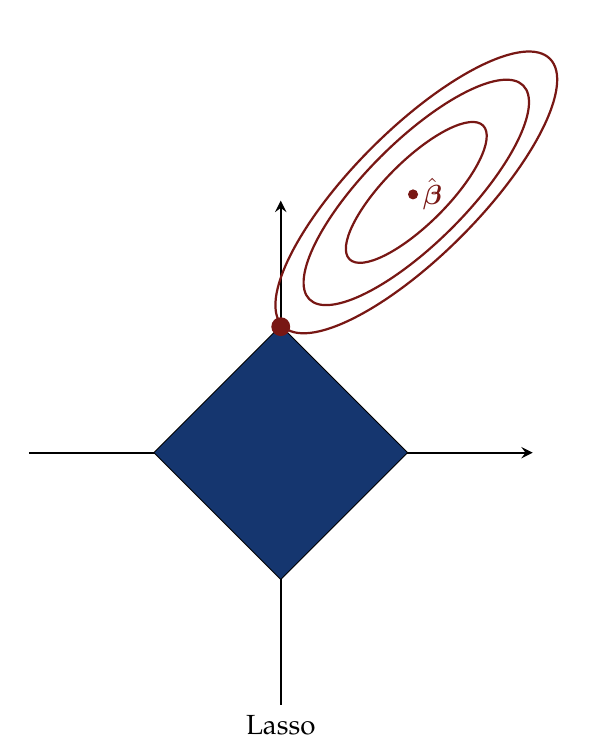
\begin{tikzpicture}[scale=1.6]
          % basics
          \draw [-stealth,color=black,thick] (0,2) -- (4,2);
          \draw [-stealth,color=black,thick] (2,0) node[below] {Lasso} -- (2,4);
          \draw [name path=lup,color=black,thick] (1,2) -- (2,3) -- (3,2);
          \draw [name path=ldown,color=black,thick]  (3,2) -- (2,1) -- (1,2);
          \draw [name path=lmid, color=black, thick] (1,2) -- (3,2);
          \tikzfillbetween[of=lup and ldown, on layer=main]{myblue};
          \draw [rotate=45, thick, color=myred] (5.05,0.7) ellipse (1.5cm and 0.5cm);
          \draw [rotate=45, thick, color=myred] (5.05,0.7) ellipse (1.2cm and 0.4cm);
          \draw [rotate=45, thick, color=myred] (5.05,0.7) ellipse (0.75cm and 0.25cm);
          \filldraw [color=myred] (3.05,4.05) circle (1pt) node[right] {$\hat{\boldsymbol{\beta}}$};
          \filldraw [color=myred] (2,3) circle (2pt);
      \end{tikzpicture}
    \end{minipage}
    \hfill
    \begin{minipage}[b]{0.45\textwidth}
        \centering
        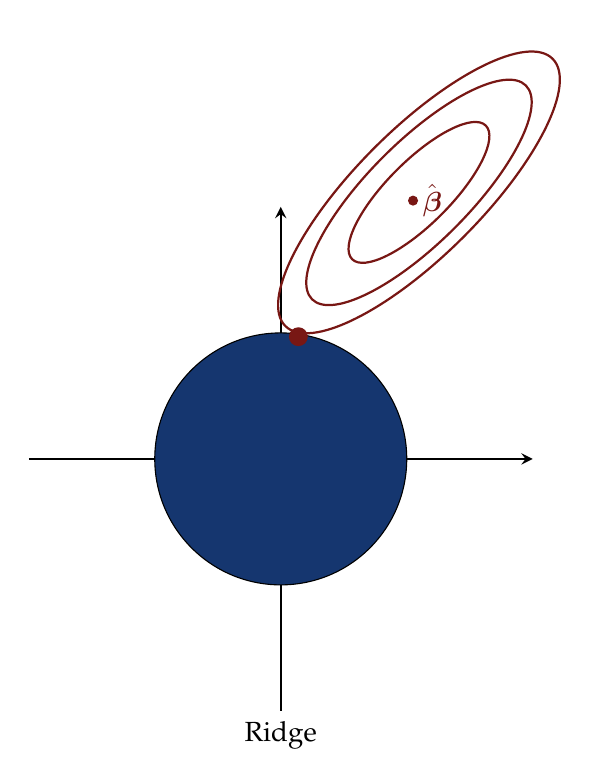
\begin{tikzpicture}[scale=1.6]
            % basics
            \draw [-stealth,color=black,thick] (0,2) -- (4,2);
            \draw [-stealth,color=black,thick] (2,0) node[below] {Ridge} -- (2,4);
            \draw [color=black,thick] (2,2) -- (2,1);
            %\draw [name path=ldown,color=black,thick]  (3,2) -- (2,1) node[right,xshift=2pt, yshift=-2pt] {Lasso} -- (1,2);
            %\draw [name path=lmid, color=black, thick] (1,2) -- (3,2);
            \node[circle,draw,minimum size=3.2cm, fill =myblue] (c) at (2,2){};
            \draw [rotate=45, thick, color=myred] (5.1,0.72) ellipse (1.5cm and 0.5cm);
            \draw [rotate=45, thick, color=myred] (5.1,0.72) ellipse (1.2cm and 0.4cm);
            \draw [rotate=45, thick, color=myred] (5.1,0.72) ellipse (0.75cm and 0.25cm);
            \filldraw [color=myred] (3.05,4.05) circle (1pt) node[right] {$\hat{\boldsymbol{\beta}}$};
            \filldraw [color=myred] (2.14,2.97) circle (2pt);
        \end{tikzpicture}
    \end{minipage}
\end{figure}


\newpage
\bibliographystyle{plainnat}
\bibliography{ref.bib}

\end{document}